\documentclass{article}
\usepackage{verbatim}
\usepackage{pdfpages}
\begin{document}
	\begin{enumerate}
		\item
		Testing:\\
		One sample output from a test run with command line arguments 5 10\\
		\verbatiminput{../chk.txt}
		Note that the number following remove is the index in the Vertex list, not the index from the original graph, starting from 0.\\
		The output shows correct execution of the program.\\
		\item 
		I conducted 1000 experiments with command line arguments 5 1000, see script test in the root directory.\\
		See plots on the next two pages.\\
		See output in pdata.csv in the root directory.\\
		It's hard to determine probability distribution of the max number of vertices removed with a small number of trials. However, a large number of trials made it hard to fit a parametric model, so I did a KDE(Kernel Density Estimate).\\
		The histogram shows that it is highly probable that the maximum number is one, since a lot of vertices are connected only to a hub vertex, and if the hub was removed, the graph could not be connected.\\
		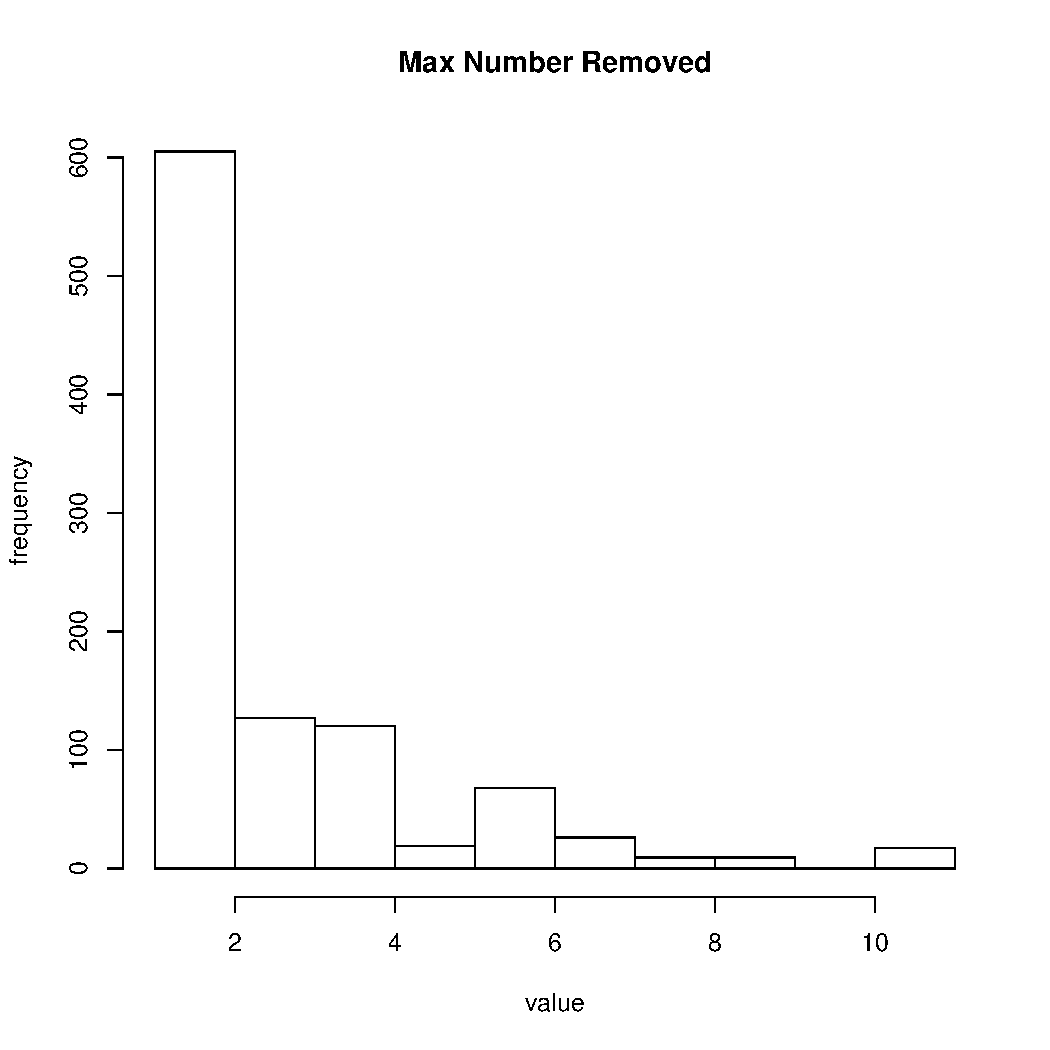
\includepdf[pages=-]{../Rplots.pdf}
		\newpage
		\item 
		Practical usages:\\
		\begin{enumerate}
			\item 
			Social Network:\\
			\begin{itemize}
				\item 
				Vertices: Individual persons\\
				\item 
				Edges: Relationships between persons\\
			\end{itemize}
			\item 
			Supply Chain Network:\\
			\begin{itemize}
				\item 
				Vertices: Individual cities\\
				\item 
				Edges: Connections between cities(All sorts of transportation)\\
			\end{itemize}
			\item 
			Power Supply Network:
			\begin{itemize}
				\item
				Vertices: Individual cities\\
				\item 
				Edges: Power lines between cities\\
			\end{itemize}
		\end{enumerate}
	\end{enumerate}
\end{document}